\documentclass[11pt]{article}
\usepackage[margin=1in]{geometry}
\usepackage[T1]{fontenc}
\usepackage{amsmath,amssymb,booktabs,graphicx,natbib,longtable,pdflscape,placeins,hyperref}
\setlength{\emergencystretch}{2em}
\hypersetup{colorlinks=true,urlcolor=blue,citecolor=blue}
\renewcommand{\thetable}{A\arabic{table}}
\renewcommand{\thefigure}{A\arabic{figure}}
\title{Supporting appendices\\Choosing price forecasts for cryptocurrency sales}
\author{Lai Jien Weng\\Monash University}\date{20 September 2026}
\begin{document}\maketitle\appendix
\section{Frozen design, features and calendar}
The experiment protocol was recorded before extracting features or computing outcomes for SOLUSDT, BNBUSDT and XRPUSDT. These are newly analysed assets in this project, but their historical dates overlap previously inspected BTC/ETH observations and common market shocks. They are not an independent prospective sample. The candidate set, costs, metrics, bootstrap and primary contrast were fixed before the run. All results, including baseline failures, are retained.

Forty Binance monthly spot archives cover five assets from 1 January through 31 August 2026, totalling 1,749,600 one-minute records \citep{binance2026}. The 24 newly acquired files supply 1,049,760 records. Archive checksums match the exchange's published SHA256 files; schema checks require complete minute grids, finite fields, positive prices, consistent OHLC, nonnegative volume and valid taker volumes. These checks do not establish order fill feasibility.

All timestamps are UTC. For each asset, the six training/calibration/evaluation triples are Jan/Feb/Mar, Feb/Mar/Apr, Mar/Apr/May, Apr/May/Jun, May/Jun/Jul and Jun/Jul/Aug, all in 2026. Each role uses its entire calendar month, from the first date at 00:00 to the last date at 23:59. February has 28 days; April and June have 30; the other months have 31. Each evaluation month follows its calibration month without refitting on calibration data.

Decision minutes have daily offsets $i=5,35,\ldots,1415$. Execution uses opens at $i+1,\ldots,i+15$, relative to open $P_i$. For example, a 00:05 decision uses completed bars opening 00:00--00:04 and executes hypothetically at 00:06--00:20. The final episode executes at 23:36--23:50. There are 48 orders per asset per date: 26,496 transfer episodes and 17,664 development episodes across the same 184 dates. Nonoverlapping execution windows do not imply independent observations.

For $h\in\{1,5\}$, imbalance is
\[
I_{h,i}=\frac{\sum_{k=i-h}^{i-1}(2V^B_k-V_k)}{\sum_{k=i-h}^{i-1}V_k},
\]
with zero for zero total volume. Returns are $R_{h,i}=10^4\log(P_i/P_{i-h})$, available at the decision-time open. Ridge uses $(I_{1,i},I_{5,i},R_{1,i},R_{5,i},\log(1+\sum_{k=i-5}^{i-1}V_k))$. Training means and standard deviations standardize these features; standard deviations below $10^{-12}$ are replaced by one.

The seven candidates, in tie order, are zero, the mean training price path, three OLS models using respectively $I_1$, $I_5$, $R_5$, and two ridge models. Every fitted model includes an intercept. For standardized training features $Z$, the ridge objective is
\[
\frac1{n_{\rm train}}\|Y-\mathbf1a^\top-ZB\|_F^2+\lambda\|B\|_F^2,
\qquad\lambda\in\{0.1,1.0\}.
\]
The intercept is unpenalized. All fifteen price horizons are fitted jointly using the same penalty, with no hyperparameter search. Forecasts include the fitted intercept, unlike the signal-only forecast in the earlier illustration.

Every selector uses the same candidates, calibration episodes and costs. Endpoint MSE scores horizon fifteen; path MSE averages all fifteen coordinates; contrast MSE subtracts each forecast path's own coordinate mean and the realized path's own mean before scoring. This centering is a validation loss, not use of future prices when placing a trade. Economic selection maximizes mean baseline-relative objective gain. A tolerance of $10^{-12}$ defines ties, resolved by the fixed candidate order. Zero is available to all rules, and no unique attenuation or rejection option is added to the economic rule.
\section{Why common price-level errors do not affect timing}
The result below follows from equality-constrained quadratic optimization, consistent with signal-dependent execution and decision-focused evaluation \citep{almgren2001,forde2022,abijaber2025,elmachtoub2022}. Write
\[
K(u)=\tfrac12u^\top Hu+g^\top u+c,
\quad H=2\eta NI+\frac{2r}{N}L^\top L,
\quad g=-\frac{2r}{N}L^\top\mathbf1.
\]
With $z=H^{-1}\mathbf1$, define $Q=H^{-1}-zz^\top/(\mathbf1^\top z)$. Then $Q\mathbf1=0$ and $QHQ=Q$. Under the equality constraint, stationarity gives $Hu+g-\mu+\lambda\mathbf1=0$. Subtracting the zero-forecast solution yields $u(\mu)=u_0+Q\mu$.

If the baseline and candidate equality solutions are nonnegative, they are also the unique simplex solutions. Since the baseline gradient is proportional to $\mathbf1$,
\[
K(u_0+Q\mu)-K(u_0)=\tfrac12\mu^\top Q\mu.
\]
The realized gain is therefore
\begin{align*}
G(\mu,p)&=\mu^\top Qp-\tfrac12\mu^\top Q\mu\\
&=\tfrac12p^\top Qp-\tfrac12(\mu-p)^\top Q(\mu-p).
\end{align*}
The first term does not depend on the candidate. With $r=0$, let $P=I-\mathbf1\mathbf1^\top/N$; then $Q=P/(2\eta N)$ and
\[
G(\mu,p)=\frac{\|Pp\|^2-\|P(\mu-p)\|^2}{4\eta N}.
\]
Maximizing mean calibration gain and minimizing demeaned-path MSE have identical exact rankings under these conditions. Numerical near ties require scale-adjusted tolerances to guarantee identical tie handling; our fixed absolute tolerances did not prevent the reported empirical agreement. The identity needs feasible equality solutions for the candidate and baseline; the hindsight price optimizer need not be feasible unless interpreting the additive term as attainable oracle gain.

When nonnegativity binds, the global quadratic forecast-error expression can fail. Exact decision regret remains valid:
\[
\mathcal L(\mu,p)=J_p(u(\mu))-J_p(u(p))\geq0,
\quad G(\mu,p)=G(p,p)-\mathcal L(\mu,p).
\]
With $d=u(\mu)-u(p)$, regret equals $\tfrac12d^\top Hd+(Hu(p)+g-p)^\top d$; the final term is nonnegative by constrained optimality and cannot generally be discarded. Hindsight actions are used only for this identity, never for selection or execution in the experiment.

The separate numerical audit checks equality-solution eligibility rather than merely checking that constrained solutions are feasible. At primary costs, 2,273 of 182,448 transfer calibration candidate-episodes have infeasible equality solutions. Only one of eighteen transfer calibration cells has all candidate equality solutions feasible. The largest numerical discrepancy in the equality-solution identity across audited costs and samples is $9.10\times10^{-13}$. Therefore the observed agreement between economic and contrast selectors is not explained by claiming that all observations satisfy the interior conditions.
\section{Complete results, dependence and heterogeneity}
The primary contrast was fixed as economic minus endpoint selection in the transfer cohort at $\eta=2,r=1$. Day aggregation averages equal numbers of observations from all three assets. The bootstrap samples circular blocks of seven consecutive dates, allowing blocks to cross month boundaries and wrap from the end to the beginning of the evaluation period. It uses 4,000 draws and seed 20260920. One- and fourteen-day results were also specified in advance. Models, coefficients and choices remain fixed, so intervals omit their estimation uncertainty. Circular block resampling and the stationary bootstrap are distinct dependence-resampling constructions \citep{politis1994}.

The primary mean difference is 0.0156367 bps with seven-day interval [0.0027791,0.0318384]. The one-day interval is [0.0057226,0.0265022]; the fourteen-day interval is [0.0008073,0.0373538]. These are conditional intervals for the frozen comparison. All other contrasts and scenario intervals are secondary and unadjusted for multiplicity.
\begin{figure}[htbp]\centering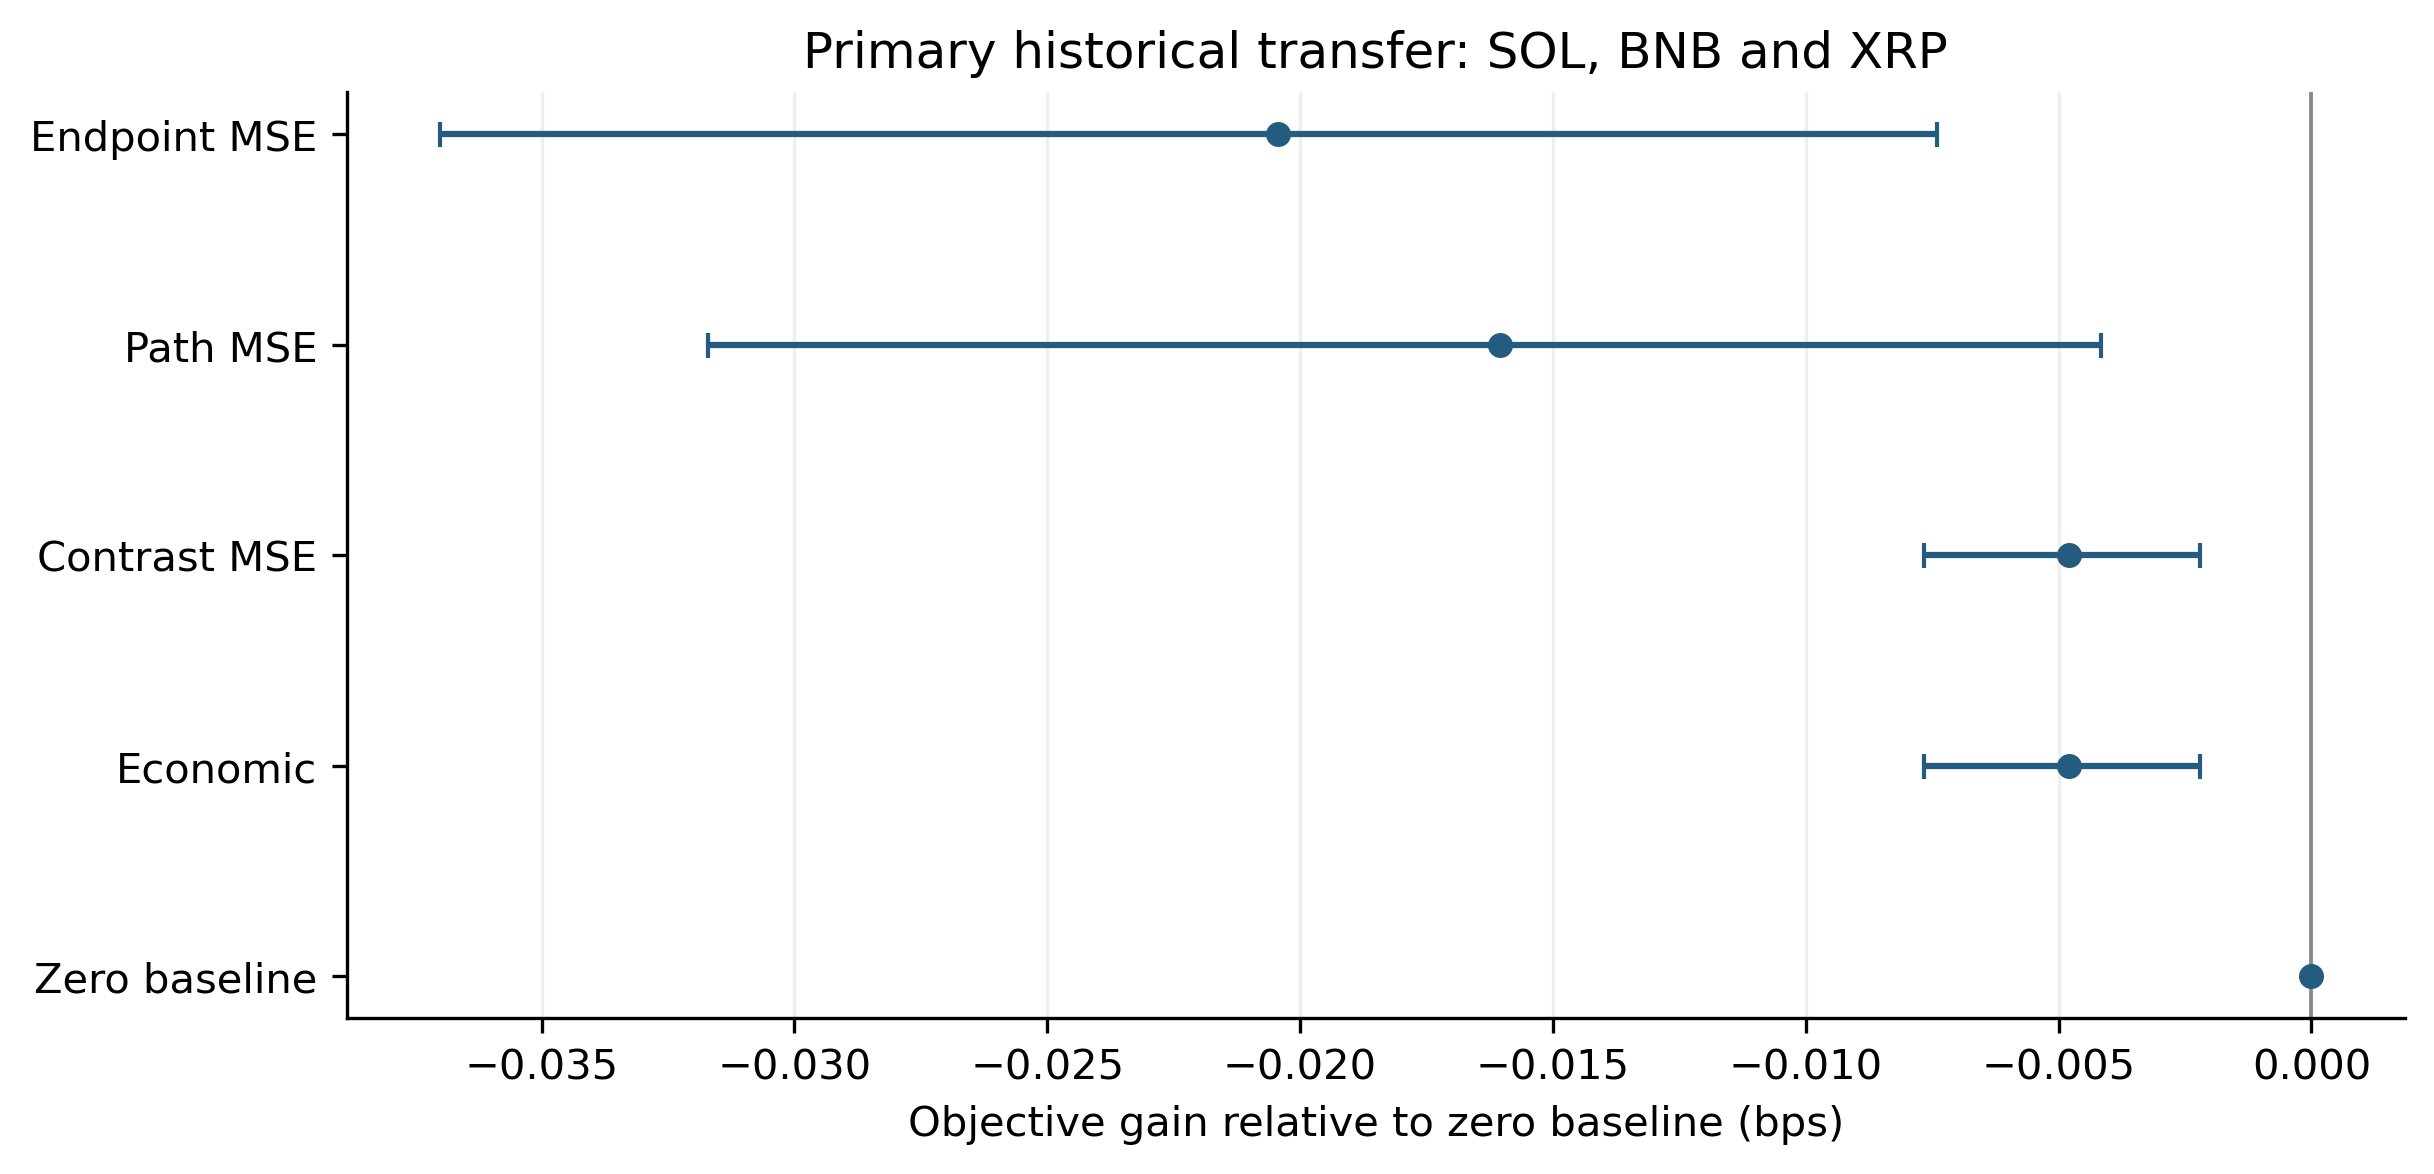
\includegraphics[width=\linewidth]{figures/transfer_selectors.png}
\caption{Primary transfer selector outcomes. Identical economic and contrast results represent the same choices, not two independent successes. All selectors underperform the no-signal baseline.}
\end{figure}
\begin{table}[htbp]\centering\small
\caption{All prespecified cost scenarios: paired economic-minus-endpoint objective gains.}
\resizebox{\linewidth}{!}{\begin{tabular}{rrrrrr}
\toprule
$\eta$ & $r$ & Endpoint gain & Economic gain & Paired difference & Conditional 95\% interval \\
\midrule
0.5 & 0 & -0.06284 & -0.01851 & 0.04432 & [0.00765, 0.08707] \\
0.5 & 1 & -0.05838 & -0.01626 & 0.04212 & [0.00771, 0.08306] \\
2 & 0 & -0.02085 & -0.00492 & 0.01592 & [0.00271, 0.03245] \\
2 & 1 & -0.02043 & -0.00479 & 0.01564 & [0.00278, 0.03184] \\
5 & 0 & -0.00894 & -0.00197 & 0.00698 & [0.00133, 0.01412] \\
5 & 1 & -0.00883 & -0.00195 & 0.00688 & [0.00134, 0.01389] \\
\bottomrule
\end{tabular}
}
\end{table}
\begin{figure}[htbp]\centering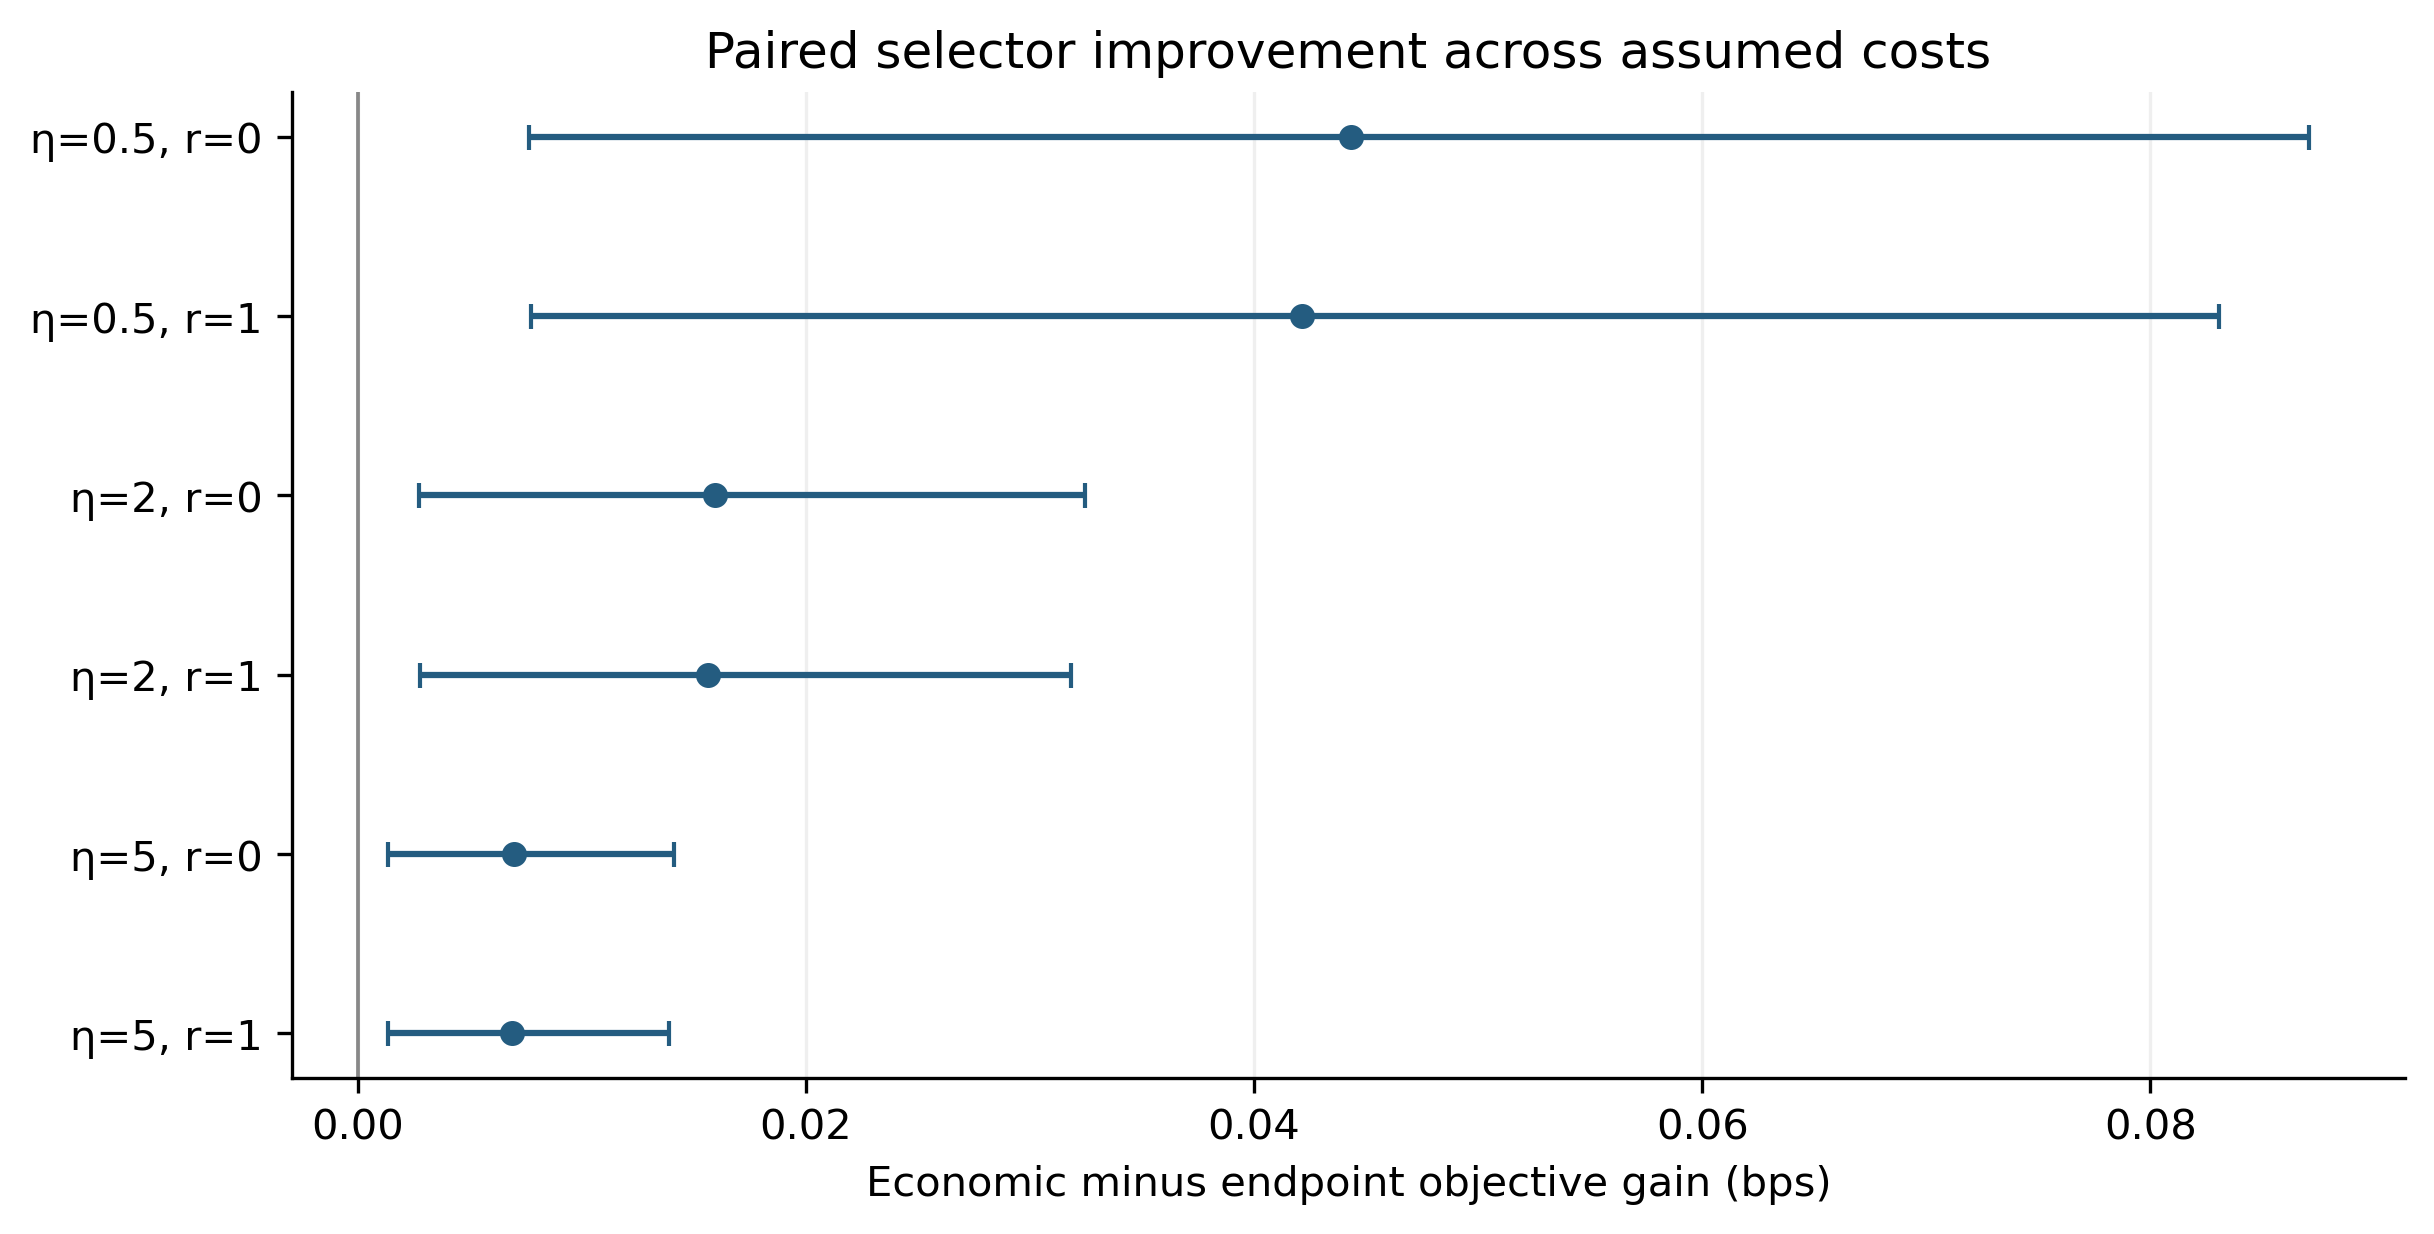
\includegraphics[width=\linewidth]{figures/transfer_cost_sensitivity.png}
\caption{Conditional seven-day block intervals for the paired difference across assumed costs. This checks sensitivity to model parameters, not calibration to observed market impact.}
\end{figure}

Per-asset primary mean differences are 0.03815 bps for SOL, 0.00494 for BNB and 0.00382 for XRP. SOL contributes about 81\% of the pooled difference, March about 79\%, and SOL in March alone about 66\%. Omitting March gives 0.00397 bps; omitting any other evaluation month also leaves a positive mean. These are descriptive influence checks without refitting, not a basis for choosing which months to retain.

Economic selection chooses the baseline in eleven of eighteen primary transfer cells. Each of the remaining seven selections loses against the baseline in evaluation. Economic selection minus baseline is $-0.0047949$ bps with interval [$-0.0076617$,$-0.0022067$]. Economic minus ordinary path MSE is 0.01125 bps with interval [$-0.000063$,0.026637], leaving superiority unresolved. On development BTC/ETH the economic-minus-endpoint mean is $-0.000771$, interval [$-0.006702$,0.003313]. These findings rule out a claim of generally superior or profitable forecasting.
\begin{table}[htbp]\centering\scriptsize
\caption{Every fixed candidate at primary costs. The table reports candidate performance without calibration selection.}
\resizebox{\linewidth}{!}{\begin{tabular}{lrrrr}
\toprule
Candidate & Development mean & 95\% interval & Transfer mean & 95\% interval \\
\midrule
zero & 0.00000 & [0.00000, 0.00000] & 0.00000 & [0.00000, 0.00000] \\
mean & -0.04989 & [-0.08150, -0.02158] & -0.04993 & [-0.08680, -0.01826] \\
flow1 & -0.06594 & [-0.10646, -0.02982] & -0.06316 & [-0.10440, -0.02717] \\
flow5 & -0.05409 & [-0.08923, -0.02237] & -0.06224 & [-0.10546, -0.02440] \\
momentum5 & -0.07269 & [-0.11027, -0.03900] & -0.08180 & [-0.12521, -0.04142] \\
ridge\_01 & -0.09410 & [-0.13396, -0.05772] & -0.12069 & [-0.16089, -0.08047] \\
ridge\_1 & -0.05748 & [-0.08838, -0.03045] & -0.07055 & [-0.10555, -0.03824] \\
\bottomrule
\end{tabular}
}
\end{table}
\FloatBarrier
\begin{landscape}
\small\setlength{\tabcolsep}{3pt}
\noindent\textbf{All primary-cost asset-month selections.} BTC and ETH are development assets; SOL, BNB and XRP are transfer assets. Month labels 03--08 refer to March--August 2026. Columns report the chosen candidate and its baseline-relative objective gain. Candidate IDs follow Appendix A. Every specified cell is shown.
\begin{longtable}{llllllrrrrr}
\toprule
Asset & Month & End ID & Path ID & Contr. ID & Econ. ID & End gain & Path gain & Contr. gain & Econ. gain & Econ.$-$End \\
\midrule
\endhead
BNB & 03 & momentum5 & momentum5 & mean & mean & -0.03312 & -0.03312 & -0.00856 & -0.00856 & 0.02456 \\
BNB & 04 & zero & zero & zero & zero & 0.00000 & 0.00000 & 0.00000 & 0.00000 & 0.00000 \\
BNB & 05 & flow5 & flow5 & zero & zero & -0.00621 & -0.00621 & 0.00000 & 0.00000 & 0.00621 \\
BNB & 06 & flow1 & flow1 & flow1 & flow1 & -0.00699 & -0.00699 & -0.00699 & -0.00699 & 0.00000 \\
BNB & 07 & momentum5 & momentum5 & zero & zero & 0.00143 & 0.00143 & 0.00000 & 0.00000 & -0.00143 \\
BNB & 08 & zero & zero & zero & zero & 0.00000 & 0.00000 & 0.00000 & 0.00000 & 0.00000 \\
BTC & 03 & flow5 & flow5 & zero & zero & -0.00499 & -0.00499 & 0.00000 & 0.00000 & 0.00499 \\
BTC & 04 & zero & zero & zero & zero & 0.00000 & 0.00000 & 0.00000 & 0.00000 & 0.00000 \\
BTC & 05 & momentum5 & mean & mean & mean & -0.01361 & -0.00896 & -0.00896 & -0.00896 & 0.00464 \\
BTC & 06 & zero & zero & zero & zero & 0.00000 & 0.00000 & 0.00000 & 0.00000 & 0.00000 \\
BTC & 07 & mean & flow5 & zero & zero & 0.00082 & 0.00049 & 0.00000 & 0.00000 & -0.00082 \\
BTC & 08 & zero & zero & zero & zero & 0.00000 & 0.00000 & 0.00000 & 0.00000 & 0.00000 \\
ETH & 03 & flow1 & flow1 & ridge\_1 & ridge\_1 & -0.02270 & -0.02270 & -0.04066 & -0.04066 & -0.01796 \\
ETH & 04 & zero & zero & zero & zero & 0.00000 & 0.00000 & 0.00000 & 0.00000 & 0.00000 \\
ETH & 05 & mean & mean & mean & mean & -0.02702 & -0.02702 & -0.02702 & -0.02702 & 0.00000 \\
ETH & 06 & zero & zero & zero & zero & 0.00000 & 0.00000 & 0.00000 & 0.00000 & 0.00000 \\
ETH & 07 & flow5 & mean & flow5 & flow5 & -0.00020 & -0.00727 & -0.00020 & -0.00020 & 0.00000 \\
ETH & 08 & zero & zero & zero & zero & 0.00000 & 0.00000 & 0.00000 & 0.00000 & 0.00000 \\
SOL & 03 & momentum5 & momentum5 & mean & mean & -0.20418 & -0.20418 & -0.02030 & -0.02030 & 0.18388 \\
SOL & 04 & zero & zero & zero & zero & 0.00000 & 0.00000 & 0.00000 & 0.00000 & 0.00000 \\
SOL & 05 & flow5 & zero & mean & mean & -0.03937 & 0.00000 & -0.01733 & -0.01733 & 0.02205 \\
SOL & 06 & zero & zero & zero & zero & 0.00000 & 0.00000 & 0.00000 & 0.00000 & 0.00000 \\
SOL & 07 & zero & flow1 & flow5 & flow5 & 0.00000 & -0.00437 & -0.02294 & -0.02294 & -0.02294 \\
SOL & 08 & ridge\_1 & zero & zero & zero & -0.04342 & 0.00000 & 0.00000 & 0.00000 & 0.04342 \\
XRP & 03 & mean & momentum5 & zero & zero & -0.01119 & -0.01384 & 0.00000 & 0.00000 & 0.01119 \\
XRP & 04 & zero & zero & zero & zero & 0.00000 & 0.00000 & 0.00000 & 0.00000 & 0.00000 \\
XRP & 05 & flow5 & mean & mean & mean & -0.01743 & -0.00593 & -0.00593 & -0.00593 & 0.01150 \\
XRP & 06 & zero & zero & zero & zero & 0.00000 & 0.00000 & 0.00000 & 0.00000 & 0.00000 \\
XRP & 07 & flow1 & momentum5 & flow1 & flow1 & -0.00357 & -0.01268 & -0.00357 & -0.00357 & 0.00000 \\
XRP & 08 & zero & zero & zero & zero & 0.00000 & 0.00000 & 0.00000 & 0.00000 & 0.00000 \\
\bottomrule
\end{longtable}

\end{landscape}
\section{Prior art and reproducibility}
\citet{kweon2024} already train liquidity forecasts for decision quality in adaptive execution. The present experiment selects among fixed price-path models and includes a demeaned-path control. It does not reproduce their algorithm or establish superiority to it. The reference was verified through institutional bibliographic metadata and the abstract; no full-text replication is claimed.

The code and frozen experiment are in \path{revisions/2026-09-20-selection/}. The protocol lock records the pre-outcome SHA256 digest. The run manifest records the analysis and validator hashes. Files include fitted coefficients, calibration scores, every selected ID, daily and episode-level gains, archive checksums, and complete scenario summaries. The maximum QP KKT residual is $1.25\times10^{-11}$.

An isolated rerun reproduced the study summary exactly after excluding only its completion timestamp; fitted coefficients and uncompressed daily and episode CSV bytes also matched exactly. Eight tests check causal feature windows, shared baseline/tie rules, evaluation-outcome isolation, objective signs, nonnegative schedules, paired resampling and the zero-inventory-penalty identity. These are numerical checks, not evidence that minute opens are executable prices. Public aggregate data are used; no live orders or participant records are involved.

Further analysis must retain the distinction between retrospective asset transfer and a prospective test. Any new predictors, cost estimates, observations or decision rules require a separately recorded design; they must not silently replace the frozen outcomes reported here.
\begingroup\raggedright\bibliographystyle{plainnat}\bibliography{references}\endgroup
\end{document}
